\documentclass{tufte-book}


% Packages to include
\usepackage{booktabs, xspace, units}
\usepackage{amsthm, amsmath, amssymb, thmtools}

% For graphics / images
\usepackage{graphicx}
\setkeys{Gin}{width=\linewidth,totalheight=\textheight,keepaspectratio}
\graphicspath{{graphics/}}


% Define subtitle command
\newcommand{\subtitle}[1]{
  \gdef\@subtitle{#1}
}


% Redefine title command to include subtitle
\renewcommand{\maketitlepage}[0]{%
  \cleardoublepage%
  {%
  \sffamily%
  \begin{fullwidth}%
  \fontsize{14}{16}\selectfont\par\noindent\textcolor{darkgray}{\allcaps{\thanklessauthor}}%
  \vspace{11.5pc}%
  \fontsize{36}{40}\selectfont\par\noindent\textcolor{darkgray}{\allcaps{\thanklesstitle}}%
  \fontsize{12}{40}\selectfont\par\noindent\textcolor{darkgray}{\allcaps{\@subtitle}}%
  \vfill%
  \fontsize{12}{14}\selectfont\par\noindent\allcaps{\thanklesspublisher}%
  \end{fullwidth}%
  }
  \thispagestyle{empty}%
  \clearpage%
}


% Book metadata
\title{Seeing Theory}
\subtitle{A Visual Introduction to Probability and Statistics}
\author{Tyler Devlin, Jingru Guo, Daniel Kunin, Dan Xiang}
\publisher{Brown University}

% Copywrite command
\newcommand{\copyrightpage}{%
    \newpage%
    \begin{fullwidth}%
    ~\vfill%
    \thispagestyle{empty}%
    \setlength{\parindent}{0pt}%
    \setlength{\parskip}{\baselineskip}%
    Copyright \copyright\ \the\year\ \thanklessauthor%
    \par\smallcaps{Published by \thanklesspublisher}%
    \par\smallcaps{students.brown.edu/seeingtheory}%
    \par Licensed under the Apache License, Version 2.0 (the ``License''); you may not
    use this file except in compliance with the License. You may obtain a copy
    of the License at \url{http://www.apache.org/licenses/LICENSE-2.0}. Unless
    required by applicable law or agreed to in writing, software distributed
    under the License is distributed on an \smallcaps{``AS IS'' BASIS, WITHOUT
    WARRANTIES OR CONDITIONS OF ANY KIND}, either express or implied. See the
    License for the specific language governing permissions and limitations
    under the License.\index{license}%
    \par\textit{First printing, \monthyear}%
    \end{fullwidth}%
}

% Prints the month name and year
\newcommand{\monthyear}{%
  \ifcase\month\or January\or February\or March\or April\or May\or June\or
  July\or August\or September\or October\or November\or
  December\fi\space\number\year
}

% Inserts a blank page
\newcommand{\blankpage}{\newpage\hbox{}\thispagestyle{empty}\newpage}


% Symbol Commands
\newcommand\ind{\mathbbm{1}}
\newcommand\complex{\mathbbm{C}}
\newcommand\real{\mathbbm{R}}
\newcommand\rational{\mathbbm{Q}}
\newcommand\nat{\mathbbm{N}}
\newcommand\integer{\mathbbm{Z}}
\newcommand\prob{\mathbbm{P}}
\newcommand\expect{\mathbbm{E}}
\newcommand\eps{\varepsilon}
\newcommand\var{\text{Var}}
\newcommand\cov{\text{Cov}}
\newcommand\hd{\texttt{H}}
\newcommand\tl{\texttt{T}}

% Theorem Commands
\theoremstyle{definition}
\newtheorem{theorem}{Theorem}
\numberwithin{theorem}{section}
\newtheorem{definition}[theorem]{Definition}
\numberwithin{definition}{section}
\newtheorem{lemma}[theorem]{Lemma}
\numberwithin{lemma}{section}
\newtheorem{corollary}[theorem]{Corollary}
\numberwithin{corollary}{section}
\newtheorem{proposition}[theorem]{Proposition}
\numberwithin{proposition}{section}
\newtheorem{remark}[theorem]{Remark}
\numberwithin{remark}{section}
\newtheorem{claim}[theorem]{Claim}
\numberwithin{claim}{section}
\newtheorem{observation}[theorem]{Observation}
\numberwithin{observation}{section}
\newtheorem{fact}[theorem]{Fact}
\numberwithin{fact}{section}
\newtheorem{assumption}[theorem]{Assumption}
\numberwithin{assumption}{section}
\newtheorem{example}[theorem]{Example}
\numberwithin{example}{section}
\newtheorem{exercise}[theorem]{Exercise}
\numberwithin{exercise}{section}



%%%%%%%%%%%%%%%%%%%%%%%%%%%%%%%%%%%%%%%%%%%%%%%%%%%%%%%%%%%%%%%%%%%%%%%%%%%%%%%%%%%%%%%%%%%%%%%%%%%%%


\begin{document}

% Title, copyright, table of contents
\frontmatter
\maketitle
\copyrightpage
\tableofcontents
\cleardoublepage


% Introduction
\chapter*{Introduction}

The prerequisites of this text are basic algebra for the earlier chapters and basic calculus for the sections on continuous distributions. \sidenote{Some familiarity with poker is also expected.} 


% Chapters
\mainmatter

\chapter*{Basic Probability}

Basic probability is an introduction to the foundational ideas in probability theory.

\chapter{Likelihood}


A \textbf{probability} is a number between 0 and 1 that describes how likely an event is to occur. When setting up an experiment, we first specify a set of outcomes, which we call the \textbf{sample space}, typically denoted with the symbol $\Omega$. Collections of items in $\Omega$ are called \textbf{events}, and to these events, we associate likelihoods, or probabilities.

Let's see how to set up sample spaces in some familiar settings.

\subsection{Sample Spaces for Coin and Dice Experiments}

\begin{example}
Imagine we are flipping a coin. The set of possible outcomes is
\begin{align*}
\Omega = \{\hd,\tl\},
\end{align*}
i.e. we can flip either a ``Heads'' or a ``Tails''. 

Now suppose we flip two coins. The set of possible outcomes becomes
\begin{align*}
\Omega = \{\hd \hd, \hd \tl, \tl \hd, \tl \tl\}.
\end{align*}
\end{example}

\begin{example}
Now suppose we are rolling a die. The sample space of a die roll is similar to that of a coin flip, except we have more outcomes. Since a typical die has 6 sides, we can write the sample space as
\begin{align*}
\Omega = \{1,2,3,4,5,6\}
\end{align*}
An example of a \textbf{subset} $A$ of $\Omega$ (we write $A \subset \Omega$) could be the set of even rolls $\{2,4,6\}$. \sidenote{Should we use the terminology of "event" and "collection" instead of "subset" which we will introduce later?}

\end{example}

\subsection{Assigning Probabilities to Dice Rolls and Coin Flips}
To each element of our sample space $\Omega$, we associate a probability. We require that the sum of the probabilities of all the outcomes in $\Omega$ must be 1. To find the probability of a subset of our sample space, we would add up the probabilities of the elements contained in that subset.

\begin{example}
Assume that the die we rolled above was a fair die. Then each of the outcomes is equally likely to occur, i.e.
\begin{align*}
P(\text{roll 1}) = P(\text{roll 2}) = P(\text{roll 3}) = P(\text{roll 4}) = P(\text{roll 5}) = P(\text{roll 6}) = \frac{1}{6}
\end{align*}
To find the probability of rolling an even number, we add up all the probabilities of the even numbers in $\Omega$. This gives us
\begin{align*}
P(\text{roll an even number}) &= P(\text{roll 2}) + P(\text{roll 4}) + P(\text{roll 6}) \\
&= \frac{1}{6} + \frac{1}{6} + \frac{1}{6} \\
&= \frac{1}{2}.
\end{align*}
\end{example}

\begin{marginfigure}
  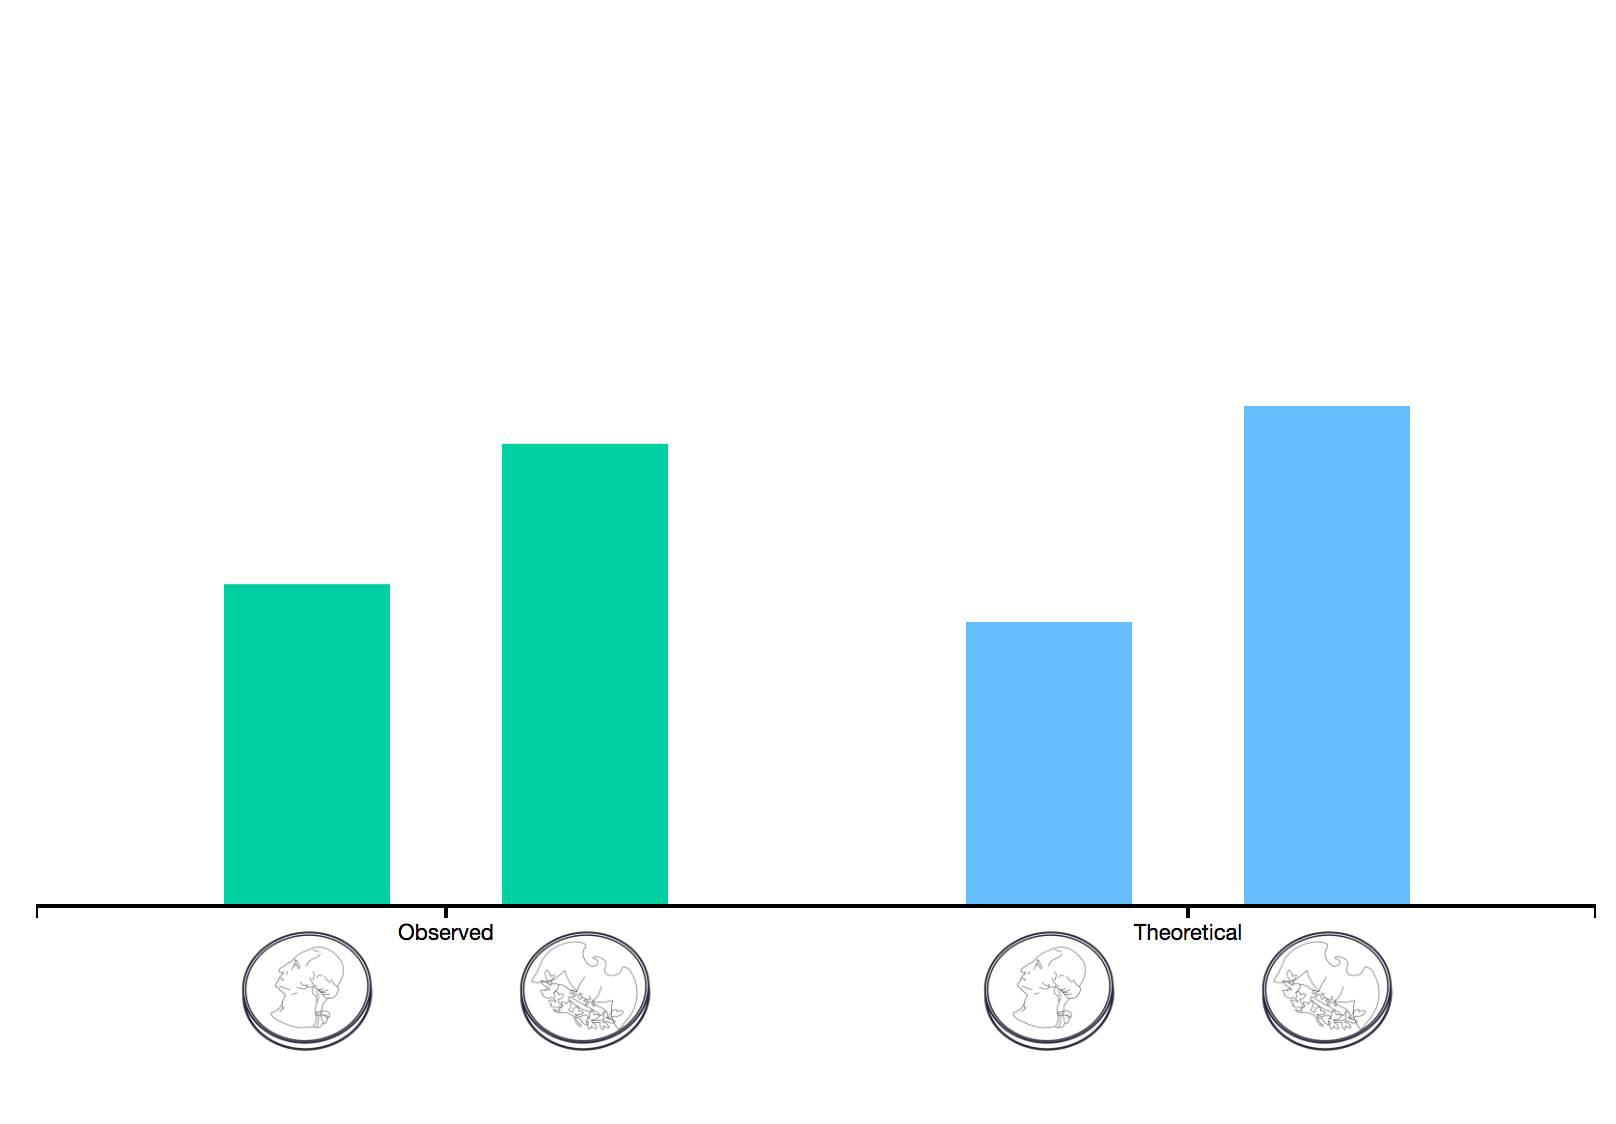
\includegraphics{likelihood.png}
  \caption{We should include screen shots directly from the visualizations}
\end{marginfigure}

\begin{example}
Suppose that we flip a single fair coin. Then as stated above, the possible outcomes are $\hd$ or $\tl$. Since it is equally likely to flip a $\hd$ as a $\tl$, we have
\begin{align*}
P(\hd) = P(\tl) = \frac{1}{2}
\end{align*}

Similarly, if we flip the coin twice, each of the possible outcomes should be equally likely, so
\begin{align*}
P(\hd \hd) = P(\hd \tl) = P(\tl \hd) = P(\tl \tl) = \frac{1}{4}
\end{align*}

Now assume that our coin has a bias, that is, the probability of flipping $\hd$ is some number between 0 and 1, denoted $p$. Then since the probabilities of all the outcomes must sum to 1, we have
\begin{align*}
P(\hd) &= p \\
P(\tl) &= 1-p
\end{align*}

Similarly, the probabilities for the second sample space become
\begin{align*}
P(\hd \hd) &= p^2 \\
P(\hd \tl) &= p (1-p) \\
P(\tl \hd) &= (1-p) p \\
P(\tl \tl) &= (1-p)^2 
\end{align*}
Since we flip a $\hd$ with probability $p$, the probability of then flipping another $\hd$ in sequence would be $p^2$. The probability of flipping a $\hd$ and then a $\tl$ is the product of their probabilities, $p\cdot (1-p)$. The last two probabilities above are obtained similarly.

We check that these probabilities sum to 1 below.
\begin{align*}
P(\hd \hd) + P(\hd \tl ) + P(\tl \hd) + P(\tl \tl) &= p^2 + p\cdot (1-p) + (1-p) 
\cdot p + (1-p)^2 \\
&= p^2 + (p - p^2) + (p - p^2) + (1 - 2p + p^2) \\
&= 2p - p^2 + (1 - 2p + p^2) \\
&= 1
\end{align*}
\end{example}


\begin{exercise}
What is the probability that we get at least one $\hd$?
\end{exercise}

\begin{proof}[Solution.]
One way to solve this problem is to add up the probabilities of all outcomes that have at least one $\hd$. We would get
\begin{align*}
P(\text{flip at least one }\hd) &= P(\hd \hd) + P(\hd \tl) + P(\tl \hd) \\
&= p^2 + p \cdot (1-p) + (1-p) \cdot p \\
&= p^2 + 2 \cdot (p-p^2) \\
&= 2p - p^2 \\
&= p \cdot (2-p).
\end{align*}
Another way to do this is to find the probability that we \textbf{don't} flip at least one $\hd$, and subtract that probability from 1. This would give us the probability that we \textbf{do} flip at least one $\hd$. 

The only outcome in which we don't flip at least one $\hd$ is if we flip $\tl$ both times. We would then compute
\begin{align*}
P(\text{don't flip at least one }\hd) = P(\tl \tl) = (1-p)^2
\end{align*}
Then to get the \textbf{complement} of this event, i.e. the event where we \textbf{do} flip at least one $\hd$, we subtract the above probability from 1. This gives us
\begin{align*}
P(\text{flip at least one } \hd) &= 1 - P(\text{don't flip at least one }\hd) \\
&= 1 - (1-p)^2 \\
&= 1 - (1 - 2p + p^2) \\
&= 2p - p^2 \\
&= p\cdot (2 - p).
\end{align*}
Wowee! Both methods for solving this problem gave the same answer. Notice that in the second calculation, we had to sum up fewer probabilities to get the answer. It can often be the case that computing the probability of the complement of an event and subtracting that from 1 to find the probability of the original event requires less work. 
\end{proof}


\subsection{Independence}
If two events $A$ and $B$ don't influence or give any information about the other, we say $A$ and $B$ are independent. Remember that this is not the same as saying $A$ and $B$ are disjoint. If $A$ and $B$ were disjoint, then given information that $A$ happened, we would know with certainty that $B$ did \textit{not} happen. Hence if $A$ and $B$ are disjoint they could never be independent. The mathematical statement of independent events is given below.

\begin{definition}
Let $A$ and $B$ both be subsets of our sample space $\Omega$. Then we say $A$ and $B$ are independent if
\begin{align*}
P(A \cap B) = P(A) P(B)
\end{align*}
In other words, if the probability of the intersection factors into the product of the probabilities of the individual events, they are independent.
\end{definition}
We haven't defined set intersection in this section, but it is defined in the set theory chapter. The $\cap$ symbol represents $A$ \textit{and} $B$ happening, i.e. the intersection of the events.

\begin{example}
Returning to our double coin flip example, our sample space was
\begin{align*}
\Omega = \{\hd \hd, \hd \tl, \tl \hd, \tl \tl\}
\end{align*}
Define the events 
\marginnote{We write the sign $\doteq$ to represent that we are defining something. In the above expression, we are defining the arbitrary symbols $A$ and $B$ to represent events.}
\begin{align*}
A &\doteq \{\text{first flip heads}\} = \{\hd \hd, \hd \tl\} \\
B &\doteq \{\text{second flip heads}\} = \{\hd \tl, \tl \tl\}
\end{align*}


Intuitively, we suspect that $A$ and $B$ are independent events, since the first flip has no effect on the outcome of the second flip. This intuition aligns with the definition given above, as
\begin{align*}
P(A \cap B) = P(\{\hd \tl\}) = \frac{1}{4}
\end{align*}
and
\begin{align*}
P(A) = P(B) = \frac{1}{4} + \frac{1}{4} = \frac{1}{2}.
\end{align*}
We can verify that
\begin{align*}
P(A \cap B) = \frac{1}{4} = \frac{1}{2} \cdot \frac{1}{2} = P(A) P(B)
\end{align*}
Hence $A$ and $B$ are independent. This may have seemed like a silly exercise, but in later chapters, we will encounter pairs of sets where it is not intuitively clear whether or not they are independent. In these cases, we can simply verify this mathematical definition to conclude independence.

\end{example}


\chapter{Expectation}
Consider the outcome of a single die roll, and call it $X$. A reasonable question one might ask is ``What is the average value of $X$?". We define this notion of ``average'' as a weighted sum of outcomes. 

Since $X$ can take on 6 values, each with probability $\frac{1}{6}$, the weighted average of these outcomes should be
\begin{align*}
\text{Weighted Average} &= \frac{1}{6} \cdot 1 + \frac{1}{6} \cdot 2 + \frac{1}{6} \cdot 3 + \frac{1}{6} \cdot 4 + \frac{1}{6} \cdot 5 + \frac{1}{6} \cdot 6 \\
&= \frac{1}{6} \cdot (1 + 2 + 3 + 4 + 5 + 6) \\
&= \frac{21}{6} \\
&= 3.5
\end{align*}
This may seem dubious to some. How can the average roll be a non-integer value? The confusion lies in the interpretation of the phrase \textit{average roll}. A more correct interpretation would be the long term average of the die rolls. Suppose we rolled the die many times, and recorded each roll. Then we took the average of all those rolls. This average would be the fraction of 1's, times 1, plus the fraction of 2's, times 2, plus the fraction of 3's, times 3, and so on. But this is exactly the computation we have done above! In the long run, the fraction of each of these outcomes is nothing but their probability, in this case, $\frac{1}{6}$ for each of the 6 outcomes.

From this very specific die rolling example, we can abstract the notion of the \textit{average value} of a random quantity. The concept of average value is an important one in statistics, so much so that it even gets a special bold faced name. Below is the mathematical definition for the \textbf{expectation}, or average value, of a random quantity $X$.

\begin{definition}
The \textbf{expected value}, or \textbf{expectation} of $X$, denoted by $E(X)$, is defined to be
\begin{align*}
E(X) = \sum_{x \in X(\Omega)}  x P(X = x)
\end{align*}
\end{definition}
This expression may look intimidating, but it is actually conveying a very simple set of instructions, the same ones we followed to compute the average value of $X$.

The $\sum$ sign means to sum over, and the indices of the items we are summing are denoted below the $\sum$ sign. The $\in$ symbol is shorthand for ``contained in'', so the expression below the $\sum$ is telling us to sum over all items \textit{contained in} our sample space $\Omega$. We can think of the expression to the right of the $\sum$ sign as the actual items we are summing, in this case, the weighted contribution of each item in our sample space.

The notation $X(\Omega)$ is used to deal with the fact that $\Omega$ may not be a set of numbers, so a weighted sum of elements in $\Omega$ isn't even well defined. For instance, in the case of a coin flip, how can we compute $\hd \cdot \frac{1}{2} + \tl \cdot \frac{1}{2}$? We would first need to assign \textit{numerical values} to $\hd$ and $\tl$ in order to compute a meaningful expected value. For a coin flip we typically make the following assignments,
\begin{align*}
\tl \mapsto 0 \\
\hd \mapsto 1 
\end{align*}
So when computing an expectation, the indices that we would sum over are contained in the set
\begin{align*}
X(\Omega) = \{0,1\}
\end{align*}
Let's use this set of instructions to compute the expected value for a coin flip.

\subsection{Expectation of a Coin Flip}
Now let $X$ denote the value of a coin flip with bias $p$. That is, with probability $p$ we flip $\hd$, and in this case we say $X = 1$. Similarly, with probability $1-p$ we flip $\tl$, and in this case we say $X = 0$. The expected value of the random quantity $X$ is then
\begin{align*}
E(X) &= \sum_{x \in X(\Omega)} x P(X = x) \\
&= \sum_{x \in \{0,1\}} x P(X = x) \\
&= 0 \cdot P(X = 0) + 1 \cdot P(X = 1) \\
&= 0 \cdot P(\tl) + 1 \cdot P(\hd) \\
&= 0 \cdot (1-p) + 1 \cdot p \\
&= p
\end{align*}
So the expected value of this experiment is $p$. If we were flipping a fair coin, then $p = \frac{1}{2}$, so the average value of $X$ would be $\frac{1}{2}$.

Again, we can never get an outcome that would yield $X = \frac{1}{2}$, but this is not the interpretation of the expectation of $X$. Remember, the correct interpretation is to consider what would happen if we flipped the coin many times, obtained a sequence of 0's and 1's, and took the average of those values. We would expect around half of the flips to give 0 and the other half to give 1, giving an average value of $\frac{1}{2}$.

\begin{exercise}
Show the following properties of expectation.
\begin{enumerate}[(a)]
\item If $X$ and $Y$ are two random variables, then
\begin{align*}
E(X + Y) = E(X) + E(Y)
\end{align*}

\item If $X$ is a random variable and $c$ is a constant, then
\begin{align*}
E(cX) = cE(X)
\end{align*}

\item If $X$ and $Y$ are independent random variables, then
\begin{align*}
    E[XY] = E[X]E[Y]
\end{align*}
\end{enumerate}
\end{exercise}

\begin{proof}
For now, we will take (a) and (c) as a fact, since we don't know enough to prove them yet (and we haven't even defined independence of random variables!). (b) follows directly from the definition of expectation given above.
\end{proof}

\begin{figure}
  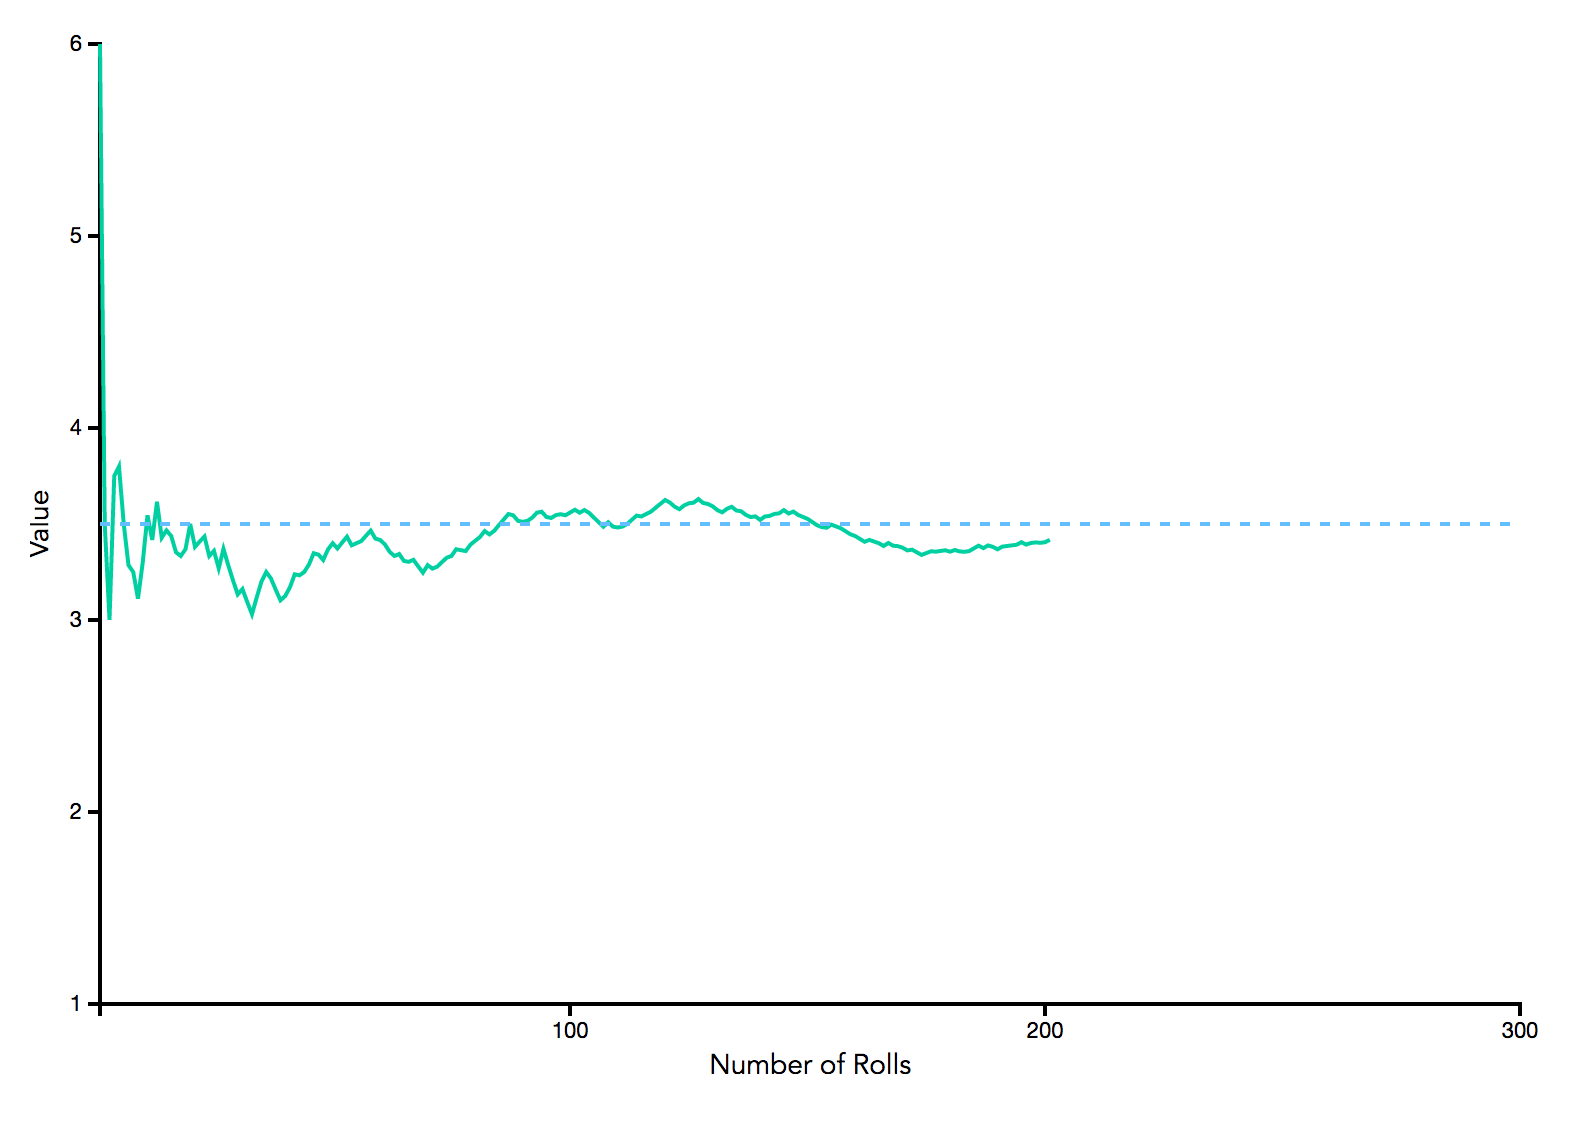
\includegraphics{expectation.png}
  \caption{We can also include images in the main body of the text}
\end{figure}

\chapter{Variance}

The variance of a random variable $X$ is a nonnegative number that summarizes on average how much $X$ differs from its mean, or expectation. The first expression that comes to mind is 
\begin{align*}
X - E(X)
\end{align*}
i.e. the difference between $X$ and its mean. This itself is a random variable, since even though $EX$ is just a number, $X$ is still random. Hence we would need to take an expectation to turn this expression into the average amount by which $X$ differs from its expected value. This leads us to
\begin{align*}
E(X-EX)
\end{align*}
This is almost the definition for variance. We require that the variance always be nonnegative, so the expression inside the expectation should always be $\geq 0$. Instead of taking the expectation of the difference, we take the expectation of the squared difference.

\begin{definition}
The \textbf{variance} of $X$, denoted by $\var(X)$ is defined 
\begin{align*}
\var(X) = E[(X - EX)^2]
\end{align*}
\end{definition}
Below we give and prove some useful properties of the variance.
\begin{proposition}
If $X$ is a random variable with mean $EX$ and $c \in \real$ is a real number,
\begin{enumerate}[(a)]
\item $\var(X) \geq 0$.

\item $\var(cX) = c^2 \var(X)$.

\item $\var(X) = E(X^2) - E(X)$.

\item If $X$ and $Y$ are independent random variables, then
\begin{align*}
    \var(X + Y) = \var(X) + \var(Y)
\end{align*}
\end{enumerate}
\end{proposition}

\begin{proof}
$ $
\begin{enumerate}[(a)]
\item Since $(X - EX)^2 \geq 0$, its average is also $\geq 0$. Hence $E[(X - EX)^2] \geq 0$.

\item Going by the definition, we have
\begin{align*}
\var(cX) &= E[(cX - E[cX])^2] \\
&= E[(cX - cEX)^2] \\
&= E[c^2(X - EX)^2 ] \\
&= c^2 E[(X - EX)^2] \\
&= c^2 \var(X)
\end{align*}

\item Expanding out the square in the definition of variance gives
\begin{align*}
\var(X) &= E[(X - EX)^2] \\
&= E[X^2 - 2XEX + (EX)^2] \\
&= E[X^2] - E(2XEX) + E((EX)^2) \\
&= E[X^2] - 2EXEX + (EX)^2 \\
&= E[X^2] - (EX)^2
\end{align*}
where the third equality comes from linearity of $E$ (Exercise 2.3 (a)) and the fourth equality comes from Exercise 2.3 (b) and the fact that since $EX$ and $(EX)^2$ are constants, their expectations are just $EX$ and $(EX)^2$ respectively.

\item By the definition of variance,
\begin{align*}
    \var(X+Y) &= E[(X+Y)^2] - (E[X+Y])^2 \\
    &= E[X^2 + 2XY + Y^2] - \Big((E[X])^2 + 2E[X]E[Y] + (E[Y])^2\Big) \\
    &= E[X^2] - (E[X])^2 + E[Y^2] - (E[Y]^2) + 2E[XY] - 2E[X]E[Y] \\
    &= E[X^2] - (E[X])^2 + E[Y^2] - (E[Y]^2) \\
    &= \var(X) + \var(Y)
\end{align*}
where the fourth equality comes from the fact that if $X$ and $Y$ are independent, then $E[XY] = E[X]E[Y]$. Independence of random variables will be discussed in the ``Random Variables'' section, so don't worry if this proof doesn't make any sense to you yet.
\end{enumerate}
\end{proof}

\begin{exercise}
Compute the variance of a die roll, i.e. a uniform random variable over the sample space $\Omega =\{1,2,3,4,5,6\}$.
\end{exercise}
\begin{proof}[Solution.]
Let $X$ denote the outcome of the die roll. By definition, the variance is
\begin{align*}
\var(X) &= E[(X-EX)]^2 \\
&= E(X^2) - (EX)^2 &&(\text{Proposition 2.11 (c)}) \\ 
&= \Big(\sum_{k=1}^6 k^2 \cdot \frac{1}{6} \Big) - (3.5)^2 &&\text{(Definition of Expectation)} \\
&= \frac{1}{6} \cdot (1 + 4 + 9 + 16 + 25 + 36) - 3.5^2 \\
&= \frac{1}{6} \cdot 91 - 3.5^2 \\
&\approx 2.92
\end{align*}

\end{proof}

\begin{remark} The square root of the variance is called the \textbf{standard deviation}.
\end{remark}

\subsection{Markov's Inequality}
Here we introduce an inequality that will be useful to us in the next section. Feel free to skip this section and return to it when you read ``Chebyschev's inequality" and don't know what's going on.

Markov's inequality is a bound on the probability that a nonnegative random variable $X$ exceeds some number $a$. 

\begin{theorem}[Markov's inequality]
Suppose $X$ is a nonnegative random variable and $a \in \real$ is a positive constant. Then
\begin{align*}
P(X \geq a) \leq \frac{EX}{a}
\end{align*}
\end{theorem}

\begin{proof}
By definition of expectation, we have
\begin{align*}
EX &= \sum_{k \in X(\Omega)} k P(X = k) \\
&= \sum_{k \in X(\Omega)\text{ s.t. } k \geq a} k P(X = k) + \sum_{k \in X(\Omega)\text{ s.t. } k < a} k P(X = k) \\
&\geq \sum_{k \in X(\Omega)\text{ s.t. } k \geq a} k P(X = k) \\
&\geq \sum_{k \in X(\Omega)\text{ s.t. } k \geq a} a P(X = k) \\ 
&= a \sum_{k \in X(\Omega)\text{ s.t. } k \geq a}  P(X = k) \\ 
&= a P(X \geq a)
\end{align*}
where the first inequality follows from the fact that $X$ is nonnegative and probabilities are nonnegative, and the second inequality follows from the fact that $k \geq a$ over the set $\{k \in X(\Omega) \text{ s.t. } k \geq a\}$.\sidenote{s.t. stands for ``such that''.}

Dividing both sides by $a$, we recover
\begin{align*}
P(X \geq a) \leq \frac{EX}{a}
\end{align*}
\end{proof}

\begin{corollary}[Chebyschev's inequality]
Let $X$ be a random variable. Then
\begin{align*}
P(|X - EX| > \eps) \leq \frac{\var(X)}{\eps^2}
\end{align*}
\end{corollary}

\begin{proof}
This is marked as a corollary because we simply apply Markov's inequality to the nonnegative random variable $(X - EX)^2$. We then have
\begin{align*}
P(|X - EX| > \eps) &= P((X-EX)^2 > \eps^2) &&\text{(statements are equivalent)}\\
&\leq \frac{E[(X-EX)^2]}{\eps^2} &&\text{(Markov's inequality)} \\
&= \frac{\var(X)}{\eps^2} &&\text{(definition of variance)}
\end{align*}
\end{proof}


\chapter*{Compound Probability}
Compound probability is the probability of joint occurrence of two or more simple events.


\chapter{Set Theory}

A probability measure $P$ is a function that maps subsets of the state space $\Omega$ to numbers in the interval $[0,1]$. In order to study these functions, we need to know some basic set theory. 

\subsection{Basic Definitions}

\begin{definition}
A \textbf{set} is a collection of items, or elements, with no repeats. Usually we write a set $A$ using curly brackets and commas to distinguish elements, shown below
\begin{align*}
A = \{a_0, a_1, a_2\}
\end{align*}
In this case, $A$ is a set with three distinct elements: $a_0, a_1,$ and $a_2$. The size of the set $A$ is denoted $|A|$ and is called the \textbf{cardinality} of $A$. In this case, $|A| = 3$. The \textbf{empty set} is denoted $\varnothing$ and means
\begin{align*}
\varnothing = \{\hspace{1em}\}
\end{align*}
\end{definition}

Some essential set operations in probability are the intersection, union, and complement operators, denoted $\cap, \cup,$ and $^c$. They are defined below
\begin{definition}
\textbf{Intersection} and \textbf{Union} each take two sets in as input, and output a single set. \textbf{Complementation} takes a single set in as input and outputs a single set. If $A$ and $B$ are subsets of our sample space $\Omega$, then we write
\begin{enumerate}[(a)]
\item $A \cap B = \{x \in \Omega : x \in A \text{ and } x \in B\}$. 

\item $A \cup B = \{x \in \Omega : x \in A \text{ or } x \in B\}$.

\item $A^c = \{x \in \Omega : x \notin A\}$.
\end{enumerate}
\end{definition}

Another concept that we need to be familiar with is that of disjointness. For two sets to be disjoint, they must share no common elements, i.e. their intersection is empty.
\begin{definition}
We say two sets $A$ and $B$ are \textbf{disjoint} if
\begin{align*}
A \cap B = \varnothing
\end{align*}
\end{definition}
It turns out that if two sets $A$ and $B$ are disjoint, then we can write the probability of their union as
\begin{align*}
P(A \cup B) = P(A) + P(B)
\end{align*}


\subsection{Set Algebra}

There is a neat analogy between set algebra and regular algebra. Roughly speaking, when manipulating expressions of sets and set operations, we can see that $``\cup"$ acts like $``+"$ and $``\cap"$ acts like $``\times"$. Taking the complement of a set corresponds to taking the negative of a number. This analogy isn't perfect, however. If we considered the union of a set $A$ and its complement $A^c$, the analogy would imply that $A \cup A^c = \varnothing$, since a number plus its negative is 0. However, it is easily verified that $A \cup A^c = \Omega$ (Every element of the sample space is either in $A$ or not in $A$.)

Although the analogy isn't perfect, it can still be used as a rule of thumb for manipulating expressions like $A \cap (B \cup C)$. The number expression analogy to this set expression is $a \times (b + c)$. Hence we could write it
\begin{align*}
a \times (b + c) &= a \times b + a \times c \\
A \cap (B \cup C) &= (A \cap B) \cup (A \cap C)
\end{align*}
The second set equality is true. Remember that what we just did was not a proof, but rather a non-rigorous rule of thumb to keep in mind. We still need to actually prove this expression.


\begin{exercise}
Show that $A \cap (B \cup C) = (A \cap B) \cup (A \cap C)$.
\end{exercise}
\begin{proof}
To show set equality, we can show that the sets are contained in each other. This is usually done in two steps. 

\textbf{Step 1:} ``$\subset$''. First we will show that $A \cap (B \cup C) \subset (A \cap B) \cup (A \cap C)$. 

Select an arbitrary element in $A \cap (B \cup C)$, denoted $\omega$. Then by definition of intersection, $\omega \in A$ and $\omega \in (B \cup C)$. By definition of union, $\omega \in (B \cup C)$ means that $\omega \in B$ or $\omega \in C$. If $\omega \in B$, then since $\omega$ is also in $A$, we must have $\omega \in A \cap B$. If $\omega \in C$, then since $\omega$ is also in $A$, we must have $\omega \in A \cap C$. Thus we must have either
\begin{align*}
\omega \in A \cap B \text{ or } \omega \in A\cap C
\end{align*}
Hence, $\omega \in (A \cap B) \cup (A \cap C)$. Since $\omega$ was arbitrary, this shows that any element of $A \cap (B \cup C)$ is also an element of $(A \cap B) \cup (A \cap C)$. Thus we have shown
\begin{align*}
A \cap (B \cup C) \subset (A \cap B) \cup (A \cap C)
\end{align*}

\textbf{Step 2:} $``\supset"$. Next we will show that $(A \cap B) \cup (A \cap C) \subset A \cap (B \cup C)$.

Select an arbitrary element in $(A \cap B) \cup (A \cap C)$, denoted $\omega$. Then $\omega \in (A \cap B)$ or $\omega \in (A \cap C)$. If $\omega \in A \cap B$, then $\omega \in B$. If $\omega \in A \cap C$, then $\omega \in C$. Thus $\omega$ is in either $B$ or $C$, so $\omega \in B \cup C$. In either case, $\omega$ is also in $A$. Hence $\omega \in A \cap (B \cup C)$. Thus we have shown
\begin{align*}
(A \cap B) \cup (A \cap C) \subset A \cap (B \cup C)
\end{align*}
Since we have shown that these sets are included in each other, they must be equal. This completes the proof.
\end{proof}

On the website, plug in each of the sets $(A \cap B) \cup (A \cap C)$ and $A \cap (B \cup C)$. Observe that the highlighted region doesn't change, since the sets are the same!

\subsection{DeMorgan's Laws}
In this section, we will show two important set identities useful for manipulating expressions of sets. These rules known as DeMorgan's Laws. 

\begin{theorem}[DeMorgan's Laws]
Let $A$ and $B$ be subsets of our sample space $\Omega$. Then
\begin{enumerate}[(a)]
\item $(A \cup B)^c = A^c \cap B^c$

\item $(A \cap B)^c = A^c \cup B^c$.
\end{enumerate}
\end{theorem}

\begin{proof}
$ $
\begin{enumerate}[(a)]
\item We will show that $(A \cup B)^c$ and $A^c \cap B^c$ are contained within each other.

\textbf{Step 1:} ``$\subset$". Suppose $\omega \in (A \cup B)^c$. Then $\omega$ is not in the set $A \cup B$, i.e. in neither $A$ nor $B$. Then $\omega \in A^c$ and $\omega \in B^c$, so $\omega \in A^c \cap B^c$. Hence $(A \cup B)^c \subset A^c \cap B^c$.

\textbf{Step 2:} ``$\supset$". Suppose $\omega \in A^c \cap B^c$. Then $\omega$ is not in $A$ and $\omega$ is not in $B$. So $\omega$ is in neither $A$ nor $B$. This means $\omega$ is not in the set $(A \cup B)$, so $\omega \in (A \cup B)^c$. Hence $A^c \cap B^c \subset (A \cup B)^c$.

Since $A^c \cap B^c$ and $(A \cup B)^c$ are subsets of each other, they must be equal.

\item Left as an exercise. 
\end{enumerate}
\end{proof}

If you're looking for more exercises, there is a link on the Set Theory page on the website that links to a page with many set identities. Try to prove some of these by showing that the sets are subsets of each other, or just plug them into the website to visualize them and see that their highlighted regions are the same.

\chapter{Combinatorics}

In many problems, to find the probability of an event, we will have to count the number of outcomes in $\Omega$ which satisfy the event, and divide by $|\Omega|$, i.e. the total number of outcomes in $\Omega$. For example, to find the probability that a single die roll is even, we count the total number of even rolls, which is 3, and divide by the total number of rolls, 6. This gives a probability of $\frac{1}{2}$. But what if the event isn't as simple as ``roll an even number''? For example if we flipped 10 coins, our event could be ``flipped 3 heads total''. How could we count the number of outcomes that have 3 heads in them without listing them all out? In this section, we will discover how to count the outcomes of such an event, and generalize the solution to be able to conquer even more complex problems.

\subsection{Permutations}
Suppose there are 3 students waiting in line to buy a spicy chicken sandwich. A question we could ask is, ``How many ways can we order the students in this line?" Since there are so few students, let's just list out all possible orderings. We could have any of
\begin{align*}
\text{6 of these }\begin{cases}
(1,2,3) \\
(1,3,2) \\
(2,1,3) \\
(2,3,1) \\
(3,1,2) \\
(3,2,1) 
\end{cases}
\end{align*}
So there are 6 total possible orderings. If you look closely at the list above, you can see that there was a systematic way of listing them. We first wrote out all orderings starting with 1. Then came the orderings starting with 2, and then the ones that started with 3. In each of these groups of orderings starting with some particular student, there were two orderings. This is because once we fixed the first person in line, there were two ways to order the remaining two students. Denote $N_i$ to be the number of ways to order $i$ students. Now we observe that the number of orderings can be written
\begin{align*}
N_3 = 3 \cdot N_2
\end{align*}
since there are 3 ways to pick the first student, and $N_2$ ways to order the remaining two students. By similar reasoning,
\begin{align*}
N_2 = 2 \cdot N_1
\end{align*}
Since the number of ways to order 1 person is just 1, we have $N_1 = 1$. Hence,
\begin{align*}
N_3 = 3 \cdot N_2 = 3 \cdot (2 \cdot N_1) = 3 \cdot 2 \cdot 1 = 6
\end{align*}
which is the same as what we got when we just listed out all the orderings and counted them. 

Now suppose we want to count the number of orderings for 10 students. 10 is big enough that we can no longer just list out all possible orderings and count them. Instead, we will make use of our method above. The number of ways to order 10 students is
\begin{align*}
N_{10} = 10 \cdot N_9 = 10 \cdot (9 \cdot N_8) = \dots = 10 \cdot 9 \cdot 8 \cdot 7 \cdot ... \cdot 2 \cdot 1 = 3,628,800
\end{align*}
It would have nearly impossible for us to list out over 3 million orderings of 10 students, but we were still able to count these orderings using our neat trick. We have a special name for this operation.

\begin{definition}
The number of \textbf{permutations}, or orderings, of $n$ distinct objects is given by the \textbf{factorial} expression,
\begin{align*}
n! = n\cdot (n-1) \cdot ... \cdot 2 \cdot 1
\end{align*}
\end{definition}
The factorial symbol is an exclamation point, which is used to indicate the excitement of counting.

\subsection{Combinations}
Now that we've established a quick method of counting the number of ways to order $n$ distinct objects, let's figure out how to do our original problem. At the start of this section we asked how to count the number of ways we could flip 10 coins and have 3 of them be heads. The valid outcomes include
\begin{align*}
&(\hd,\hd,\hd,\tl,\tl,\tl,\tl,\tl,\tl,\tl) \\
&(\hd,\hd,\tl,\hd,\tl,\tl,\tl,\tl,\tl,\tl) \\
&(\hd,\hd,\tl,\tl,\hd,\tl,\tl,\tl,\tl,\tl) \\
&\hspace{1.9cm}\vdots
\end{align*}
But its not immediately clear how to count all of these, and it definitely isn't worth listing them all out. Instead let's apply the permutations trick we learned in Section 3.2.2.

Suppose we have 10 coins, 3 of which are heads up, the remaining 7 of which are tails up. Label the 3 heads as coins 1, 2, and 3. Label the 7 tails as coins 4,5,6,7,8,9, and 10. There are 10! ways to order, or permute, these 10 (now distinct) coins. However, many of these permutations correspond to the same string of $\hd$'s and $\tl$'s. For example, coins 7 and 8 are both tails, so we would be counting the two permutations
\begin{align*}
(1,2,3,4,5,6,\textbf{7},\textbf{8},9,10) \\
(1,2,3,4,5,6,\textbf{8},\textbf{7},9,10)
\end{align*}
as different, when they both correspond to the outcome
\begin{align*}
(\hd,\hd,\hd,\tl,\tl,\tl,\tl,\tl,\tl,\tl) 
\end{align*}
hence we are \textit{over counting} by just taking the factorial of 10. In fact, for the string above, we could permute the last 7 coins in the string (all tails) in 7! ways, and we would still get the same string, since they are all tails. To any particular permutation of these last 7 coins, we could permute the first 3 coins in the string (all heads) in 3! ways and still end up with the string
\begin{align*}
(\hd,\hd,\hd,\tl,\tl,\tl,\tl,\tl,\tl,\tl) 
\end{align*}
This means that to each string of $\hd$'s and $\tl$'s, we can rearrange the coins in $3!\cdot 7!$ ways without changing the actual grouping of $\hd$'s and $\tl$'s in the string. So if there are 10! total ways of ordering the labeled coins, we are counting each unique grouping of heads and tails $3!\cdot 7!$ times, when we should only be counting it once. Dividing the total number of permutations by the factor by which we over count each unique grouping of heads and tails, we find that the number of unique groupings of $\hd$'s and $\tl$'s is
\begin{align*}
\text{\# of outcomes with 3 heads and 7 tails} = \frac{10!}{3!7!}
\end{align*}
This leads us to the definition of the binomial coefficient.
\begin{definition}
The \textbf{binomial coefficient} is defined
\begin{align*}
\binom{n}{k} \doteq \frac{n!}{k! (n-k)!}
\end{align*}
\end{definition}
The binomial coefficient, denoted $\binom{n}{k}$, represents the number of ways to pick $k$ objects from $n$ objects where the ordering within the chosen $k$ objects doesn't matter. In the previous example, $n=10$ and $k=3$. We could rephrase the question as, ``How many ways can we pick 3 of our 10 coins to be heads?" The answer is then
\begin{align*}
\binom{n}{k} = \binom{10}{3} = \frac{10!}{3! (10 - 3)!} = \frac{10!}{3!7!} = 120
\end{align*}
We read the expression $\binom{n}{k}$ as ``$n$ choose $k$". Let's now apply this counting trick to make some money.

\subsection{Poker}
One application of counting includes computing probabilities of poker hands. A poker hand consists of 5 cards drawn from the deck. The order in which we receive these 5 cards is irrelevant. The number of possible hands is thus
\begin{align*}
\binom{52}{5} = \frac{52!}{5!(52 - 5)!} = 2,598,960
\end{align*}
since there are 52 cards to choose 5 cards from. 

In poker, there are types of hands that are regarded as valuable in the following order form most to least valuable.
\begin{enumerate}
\item Royal Flush: A, K, Q, J, 10 all in the same suit.
\item Straight Flush: Five cards in a sequence, all in the same suit.
\item Four of a Kind: Exactly what it sounds like.
\item Full House: 3 of a kind with a pair.
\item Flush: Any 5 cards of the same suit, but not in sequence.
\item Straight: Any 5 cards in sequence, but not all in the same suit.
\item Three of a Kind: Exactly what it sounds like.
\item Two Pair: Two pairs of cards.
\item One Pair: One pair of cards.
\item High Card: Anything else.
\end{enumerate}
Let's compute the probability of drawing some of these hands. 

\begin{exercise}
Compute the probabilities of the above hands.
\end{exercise}
\begin{proof}[Solution.]
$ $
\begin{enumerate}
\item There are only 4 ways to get this hand. Either we get the royal cards in diamonds, clubs, hearts, or spades. We can think of this has choosing 1 suit from 4 possible suits. Hence the probability of this hand is
\begin{align*}
P(\text{Royal Flush}) = \frac{\binom{4}{1}}{\binom{52}{5}} \approx 1.5 \cdot 10^{-6}
\end{align*}

\item Assuming hands like K, A, 2, 3, 4 don't count as consecutive, there are in total 10 valid consecutive sequences of 5 cards (each starts with any of A,2,\dots,10). We need to pick 1 of 10 starting values, and for each choice of a starting value, we can pick 1 of 4 suits to have them all in. This gives a total of $\binom{10}{1} \cdot \binom{4}{1} = 40$ straight flushes. However, we need to subtract out the probability of a royal flush, since one of the ten starting values we counted was 10 (10, J, Q, K, A is a royal flush). Hence the probability of this hand is
\begin{align*}
P(\text{Straight Flush}) = \frac{\binom{10}{1}  \binom{4}{1}-\binom{4}{1}}{\binom{52}{5}} \approx 1.5 \cdot 10^{-5}
\end{align*}

\item There are 13 values and only one way to get 4 of a kind for any particular value. However, for each of these ways to get 4 of a kind, the fifth card in the hand can be any of the remaining 48 cards. Formulating this in terms of our choose function, there are $\binom{13}{1}$ ways to choose the value, $\binom{12}{1}$ ways to choose the fifth card's value, and $\binom{4}{1}$ ways to choose the suit of the fifth card. Hence the probability of such a hand is
\begin{align*}
P(\text{Four of a Kind}) = \frac{\binom{13}{1}\binom{12}{1}\binom{4}{1}}{\binom{52}{5}} \approx 0.00024
\end{align*}

\item For the full house, there are $\binom{13}{1}$ ways to pick the value of the triple, $\binom{4}{3}$ ways to choose which 3 of the 4 suits to include in the triple, $\binom{12}{1}$ ways to pick the value of the double, and $\binom{4}{2}$ ways to choose which 2 of the 4 suits to include in the double. Hence the probability of this hand is
\begin{align*}
P(\text{Full House}) = \frac{\binom{13}{1} \binom{4}{3} \binom{12}{1}\binom{4}{2}}{\binom{52}{5}} \approx 0.0014
\end{align*}

\item through 10. are left as exercises. The answers can be checked on the Wikipedia page titled ``Poker probability''.


\end{enumerate}

\end{proof}

\chapter{Conditional Probability}

Suppose we had a bag that contained two coins. One coin is a fair coin, and the other has a bias of $0.95$, that is, if you flip this biased coin, it will come up heads with probability 0.95 and tails with probability 0.05. Holding the bag in one hand, you blindly reach in with your other, and pick out a coin. You flip this coin 3 times and see that all three times, the coin came up heads. You suspect that this coin is ``likely'' the biased coin, but how ``likely'' is it?

This problem highlights a typical situation in which new information changes the likelihood of an event. The original event was ``we pick the biased coin''. Before reaching in to grab a coin and then flipping it, we would reason that the probability of this event occurring (picking the biased coin) is $\frac{1}{2}$. After flipping the coin a couple of times and seeing that it landed heads all three times, we gain new information, and our probability should no longer be $\frac{1}{2}$. In fact, it should be much higher. In this case, we ``condition'' on the event of flipping 3 heads out of 3 total flips. We would write this new probability as
\begin{align*}
P(\text{picking the biased coin} \mid \text{flipping 3 heads out of 3 total flips})
\end{align*}
The ``bar'' between the two events in the probability expression above represents ``conditioned on'', and is defined below.
\begin{definition}
The probability of an event $A$ conditioned on an event $B$ is denoted and defined
\begin{align*}
P(A \mid B) = \frac{P(A \cap B)}{P(B)}
\end{align*}
\end{definition}
The intuition of this definition can be gained by playing with the visualization on the website. Suppose we drop a ball uniformly at random in the visualization. If we ask ``What is the probability that a ball hits the orange shelf?", we can compute this probability by simply dividing the length of the orange shelf by the length of the entire space. Now suppose we are given the information that our ball landed on the green shelf. What is the probability of landing on the orange shelf now? Our green shelf has become our ``new'' sample space, and the proportion of the green shelf that overlaps with the orange shelf is now the only region in which we could have possibly landed on the orange shelf. To compute this new conditional probability, we would divide the length of the overlapping, or ``intersecting'', regions of the orange and green shelves by the total length of the green shelf.

\subsection{Bayes Rule}
Now that we've understood where the definition of conditional probability comes from, we can use it to prove a useful identity.

\begin{theorem}[Bayes Rule]
Let $A$ and $B$ be two subsets of our sample space $\Omega$. Then
\begin{align*}
P(A \mid B) = \frac{P(B \mid A) P(A)}{P(B)}
\end{align*}
\end{theorem}

\begin{proof}
By the definition of conditional probability,
\begin{align*}
P(A \mid B) = \frac{P(A \cap B)}{P(B)}
\end{align*}
Similarly,
\begin{align*}
P(B \mid A) = \frac{P(A \cap B)}{P(A)}
\end{align*}
Multiplying both sides by $P(A)$ gives
\begin{align*}
P(B \mid A)P(A) = P(A \cap B)
\end{align*}
Plugging this into our first equation, we conclude
\begin{align*}
P(A \mid B) = \frac{P(B \mid A) P(A)}{P(B)}
\end{align*}
\end{proof}

\subsection{Coins in a Bag}
Let's return to our first example in this section and try to use our new theorem to find a solution. Define the events
\begin{align*}
A &\doteq \text{\{Picking the biased coin\}} \\
B &\doteq \text{\{Flipping 3 heads out of 3 total flips\}}
\end{align*}
We were interested in computing the probability $P(A \mid B)$. By Bayes Rule,
\begin{align*}
P(A \mid B) = \frac{P(B \mid A) P(A)}{P(B)}
\end{align*}
$P(B \mid A)$, i.e. the probability of flipping 3 heads out of 3 total flips given that we picked the biased coin, is simply $(0.95)^3 \approx 0.857$. The probability $P(A)$, i.e. the probability that we picked the biased coin is $\frac{1}{2}$ since we blindly picked a coin from the bag. Now all we need to do is compute $P(B)$, the overall probability of flipping 3 heads in this experiment. Remember from the set theory section, we can write
\begin{align*}
B = B \cap \Omega = B \cap (A \cup A^c) = (B \cap A) \cup (B \cap A^c)
\end{align*}
So
\begin{align*}
P(B) = P((B \cap A) \cup (B \cap A^c)) = P(B \cap A) + P(B \cap A^c)
\end{align*}
since the two sets $B \cap A$ and $B \cap A^c$ are disjoint. By the definition of conditional probability, we can write the above expression as
\begin{align*}
&= P(B \mid A) P(A) + P(B \mid A^c) P(A^c)
\end{align*}
We just computed $P(B \mid A)$ and $P(A)$. Similarly, the probability that we flip 3 heads given that we \textit{didn't} pick the biased coin, denoted $P(B \mid A^c)$, is the probability that we flip 3 heads given we picked the fair coin, which is simply $(\frac{1}{2})^3 = 0.125$. The event $A^c$ represents the event in which $A$ does not happen, i.e. the event that we pick the fair coin. We have $P(A^c) = 1 - P(A) = 1 - \frac{1}{2} = \frac{1}{2}$. Hence
\begin{align*}
P(B) &= P(B \mid A) P(A) + P(B \mid A^c) P(A^c) \\
&= 0.857 \cdot 0.5 + 0.125 \cdot 0.5 \\
&= 0.491
\end{align*}
Plugging this back into the formula given by Bayes Rule,
\begin{align*}
P(A \mid B) = \frac{0.857 \cdot 0.5}{0.491} = 0.873
\end{align*}
Thus, given that we flipped 3 heads out of a total 3 flips, the probability that we picked the biased coin is roughly $87.3\%$.

\subsection{Conditional Poker Probabilities}
Within a game of poker, there are many opportunities to flex our knowledge of conditional probability. For instance, the probability of drawing a full house is 0.0014, which is less than 2\%. But suppose we draw three cards and find that we have already achieved a pair. Now the probability of drawing a full house is higher than 0.0014. How much higher you ask? With our new knowledge of conditional probability, this question is easy to answer. We define the events
\begin{align*}
A &\doteq \{\text{Drawing a Full House}\} \\
B &\doteq \{\text{Drawing a Pair within the first three cards}\}
\end{align*}
By Bayes Rule,
\begin{align*}
P(A \mid B) = \frac{P(B \mid A) P(A)}{P(B)}
\end{align*}
$P(B \mid A)$, i.e. the probability that we draw a pair within the first three cards given that we drew a full house eventually, is 1. This is because every grouping of three cards within a full house must contain a pair. From Section 3.2.3, the probability of drawing a full house is $P(A) = 0.0014$. 

It remains to compute $P(B)$, the probability that we draw a pair within the first three cards. The total number of ways to choose 3 cards from 52 is $\binom{52}{3}$. The number of ways to choose 3 cards containing a pair is $\binom{13}{1} \binom{4}{2} \binom{50}{1}$. There are $\binom{13}{1}$ to choose the value of the pair, $\binom{4}{2}$ ways to pick which two suits of the chosen value make the pair, and $\binom{50}{1}$ ways to pick the last card from the remaining 50 cards. Hence the probability of the event $B$ is
\begin{align*}
P(B) = \frac{\binom{13}{1} \binom{4}{2} \binom{50}{1}}{\binom{52}{3}} \approx 0.176
\end{align*}
Plugging this into our formula from Bayes Rule,
\begin{align*}
P(A \mid B) = \frac{1 \cdot 0.0014}{0.176} \approx 0.00795
\end{align*}
It follows that our chance of drawing a full house has more than quadrupled, increasing from less than 2\% to almost 8\%. 


\chapter*{Distributions}

Throughout the past chapters, we've actually already encountered many of the topics in this section. In order to define things like expectation and variance, we introduced random variables denoted $X$ or $Y$ as mappings from the sample space to the real numbers. All of the distributions we've so far looked at have been what are called \textit{discrete} distributions. We will soon look at the distinction between discrete and continuous distributions. Additionally we will introduce perhaps the most influential theorem in statistics, the \textit{Central Limit Theorem}, and give some applications.



\chapter{Random Variable}

In Section 2.2 (Expectation), we wanted to find the expectation of a coin flip. Since the expectation is defined as a weighted sum of outcomes, we needed to turn the outcomes into numbers before taking the weighted average. We provided the mapping
\begin{align*}
\tl &\mapsto 0 \\
\hd &\mapsto 1
\end{align*}
Here was our first encounter of a random variable. 
\begin{definition}
A function $X$ that maps outcomes in our sample space to real numbers, written $X : \Omega \to \real$, is called a \textbf{random variable}.
\end{definition}
In the above example, our sample space was
\begin{align*}
\Omega = \{\hd , \tl\}
\end{align*}
and our random variable $X : \Omega \to \real$, i.e. our function from the sample space $\Omega$ to the real numbers $\real$, was defined by
\begin{align*}
X(\tl) = 0 \\
X(\hd) = 1
\end{align*}
Now would be a great time to go onto the website and play with the ``Random Variable'' visualization. The sample space is represented by a hexagonal grid. Highlight some hexagons and specify the value your random variable $X$ assigns to those hexagons. Start sampling on the grid to see the empirical frequencies on the left.

%In the case of die rolling, our sample space was
%\begin{align*}
%\Omega = \{1,2,3,4,5,6\}
%\end{align*}
%and our random variable $X$ was given by the identity map, i.e.
%\begin{align*}
%X(i) = i
%\end{align*}
%for $i \in \Omega$.

\subsection{Independence of Random Variables}
In previous sections we've mentioned independence of random variables, but we've always swept it under the rug during proofs since we hadn't yet formally defined the concept of a random variable. Now that we've done so, we can finally define a second form of independence (different from independence of \textit{events}).
\begin{definition}
Suppose $X$ and $Y$ are two random variables defined on some sample space $\Omega$. We say $X$ and $Y$ are \textbf{independent random variables} if 
\begin{align*}
P(X \in A, Y \in B) = P(X \in A) P(Y \in B)
\end{align*}
for any two subsets $A$ and $B$ of $\real$.
\end{definition}
Let's go back and prove Exercise 2.9 (c), i.e. that if $X$ and $Y$ are independent random variables, then
\begin{align*}
E[XY] = E[X]E[Y]
\end{align*}
\begin{proof}
Define the random variable $Z(\omega) = X(\omega) Y(\omega)$. By the definition of expectation, the left hand side can be written
\begin{align*}
E[XY] &= \sum_{z \in Z(\Omega)} z \cdot P(Z = z) \\
&= \sum_{x \in X(\Omega), y \in Y(\Omega)} xy P(X = x, Y = y) \\
&= \sum_{x \in X(\Omega)} \sum_{y \in Y(\Omega)} xy P(X \in \{x\}, Y \in \{y\}) \\
&= \sum_{x \in X(\Omega)} \sum_{y \in Y(\Omega)} xy P(X \in \{x\})P(Y \in \{y\}) \\
&= \sum_{x \in X(\Omega)} x P(X \in \{x\}) \sum_{y \in Y(\Omega)} yP(Y \in \{y\}) \\
&= E[X]E[Y]
\end{align*}
This completes the proof.
\end{proof}

\chapter{Discrete and Continuous}

Thus far we have only studied discrete random variables, i.e. random variables that take on only up to \textit{countably} many values. The word ``countably'' refers to a property of a set. We say a set is \textit{countable} if we can describe a method to list out all the elements in the set such that for any particular element in the set, if we wait long enough in our listing process, we will eventually get to that element. In contrast, a set is called \textit{uncountable} if we cannot provide such a method. 

\subsection{Countable vs. Uncountable}
Let's first look at some examples.

\begin{example}
The set of all natural numbers
\begin{align*}
\nat \doteq \{1,2,3,\dots\}
\end{align*}
is countable. Our method of enumeration could simply be to start at 1 and add 1 every iteration. Then for any fixed element $n \in \nat$, this process would eventually reach and list out $n$.
\end{example}

\begin{example}
The integers,
\begin{align*}
\mathbb{Z} \doteq \{0,1,-1,2,-2,3,-3,\dots\}
\end{align*}
is countable. Our method of enumeration as displayed above is to start with 0 for the first element, add 1 to get the next element, multiply by -1 to get the third element, and so on. Any integer $k \in \mathbb{Z}$, if we continue this process long enough, will be reached.
\end{example}

\begin{example}
The set of real numbers in the interval $[0,1]$ is uncountable. To see this, suppose for the sake of contradiction that this set were countable. Then there would exist some enumeration of the numbers in decimal form. It might look like
\begin{align*}
&0 \hspace{.5em}.\hspace{.5em}1\hspace{.5em} 3\hspace{.5em} 5\hspace{.5em} 4 \hspace{.5em}2\hspace{.5em} 9\hspace{.5em} 5 \dots \\
&0 \hspace{.5em}.\hspace{.5em}4\hspace{.5em} 2\hspace{.5em} 9\hspace{.5em} 4 \hspace{.5em}7\hspace{.5em} 2\hspace{.5em} 6 \dots \\
&0 \hspace{.5em}.\hspace{.5em}3\hspace{.5em} 9\hspace{.5em} 1\hspace{.5em} 6 \hspace{.5em}8\hspace{.5em} 3\hspace{.5em} 1 \dots \\
&0 \hspace{.5em}.\hspace{.5em}9\hspace{.5em} 8\hspace{.5em} 7\hspace{.5em} 3 \hspace{.5em}4\hspace{.5em} 3\hspace{.5em} 5 \dots \\
&0 \hspace{.5em}.\hspace{.5em}2\hspace{.5em} 9\hspace{.5em} 1\hspace{.5em} 8 \hspace{.5em}1\hspace{.5em} 3\hspace{.5em} 6 \dots \\
&0 \hspace{.5em}.\hspace{.5em}3\hspace{.5em} 7\hspace{.5em} 1\hspace{.5em} 6 \hspace{.5em}1\hspace{.5em} 8\hspace{.5em} 2 \dots \\
&\vdots
\end{align*}
Consider the element along the diagonal of such an enumeration. In this case the number is
\begin{align*}
a \doteq 0.121318\dots
\end{align*}
Now consider the number obtained by adding 1 to each of the decimal places, i.e.
\begin{align*}
a' \doteq 0.232429\dots
\end{align*}
This number is still contained in the interval $[0,1]$, but does not show up in the enumeration. To see this, observe that $a'$ is not equal to the first element, since it differs in the first decimal place by 1. Similarly, it is not equal to the second element, as $a'$ differs from this number by 1 in the second decimal place. Continuing this reasoning, we conclude that $a'$ differs from the $n^{th}$ element in this enumeration in the $n^{th}$ decimal place by 1. It follows that if we continue listing out numbers this way, we will \textit{never} reach the number $a'$. This is a contradiction since we initially assumed that our enumeration would \textit{eventually} get to every number in $[0,1]$. Hence the set of numbers in $[0,1]$ is uncountable.
\end{example}

If you're left feeling confused after these examples, the important take away is that an uncountable set is \textit{much} bigger than a countable set. Although both are infinite sets of elements, uncountable infinity refers to a ``bigger'' notion of infinity, one which has no gaps and can be visualized as a continuum.

\subsection{Discrete Distributions}
\begin{definition}
A random variable $X$ is called \textbf{discrete} if $X$ can only take on finitely many or countably many values.
\end{definition}
For example, our coin flip example yielded a random variable $X$ which could only take values in the set $\{0,1\}$. Hence, $X$ was a discrete random variable. However, discrete random variables can still take on infinitely many values, as we see below.

\begin{example}[Poisson Distribution]
A useful distribution for modeling many real world problems is the \textit{Poisson Distribution}. Suppose $\lambda > 0$ is a positive real number. Let $X$ be distributed according to a Poisson distribution with parameter $\lambda$, i.e.
\begin{align*}
P(X = k) = \frac{e^{-\lambda}\lambda^k}{k!}
\end{align*}
where $k \in \nat$. The shorthand for stating such a distribution is $X \sim$ Poi$(\lambda)$. Since $k$ can be any number in $\nat$, our random variable $X$ has a positive probability on infinitely many numbers. However, since $\nat$ is countable, $X$ is still considered a discrete random variable. 

On the website there is an option to select the ``Poisson'' distribution in order to visualize its probability mass function. Changing the value of $\lambda$ changes the probability mass function, since $\lambda$ shows up in the probability expression above. Drag the value of $\lambda$ from 0.01 up to 10 to see how varying $\lambda$ changes the probabilities.
\end{example}

\begin{example}[Binomial Distribution]
Another useful distribution is called the \textit{Binomial Distribution}. Consider $n$ coin flips, i.e. $n$ random variables $X_1,\dots,X_n$ each of the form
\begin{align*}
X_i = \begin{cases}
1 \hspace{1em} &\text{with probability }p\\
0 &\text{with probability }1-p
\end{cases}
\end{align*}
Now consider the random variable defined by summing all of these coin flips, i.e.
\begin{align*}
S \doteq \sum_{i=1}^n X_i
\end{align*}
We might then ask, ``What is the probability distribution of $S$?'' Based on the definition of $S$, it can take on values from $0$ to $n$, however it can only take on the value 0 if all the coins end up tails. Similarly, it can only take on the value $n$ if all the coins end up heads. But to take on the value 1, we only need one of the coins to end up heads and the rest to end up tails. This can be achieved in many ways. In fact, there are $\binom{n}{1}$ ways to pick which coin gets to be heads up. Similarly, for $S = 2$, there are $\binom{n}{2}$ ways to pick which two coins get to be heads up. It follows that for $S = k$, there are $\binom{n}{k}$ ways to pick which $k$ coins get to be heads up. This leads to the following form,
\begin{align*}
P(S = k) = \binom{n}{k}p^k(1-p)^{n-k}
\end{align*}
The $p^k$ comes from the $k$ coins having to end up heads, and the $(1-p)^{n-k}$ comes from the remaining $n-k$ coins having to end up tails. Here it is clear that $k$ ranges from $0$ to $n$, since the smallest value is achieved when no coins land heads up, and the largest number is achieved when all coins land heads up. Any value between $0$ and $n$ can be achieved by picking a subset of the $n$ coins to be heads up.

Selecting the ``Binomial'' distribution on the website will allow you to visualize the probability mass function of $S$. Play around with $n$ and $p$ to see how this affects the probability distribution.
\end{example}

\subsection{Continuous Distributions}
\begin{definition}
We say that $X$ is a \textbf{continuous} random variable if $X$ can take on uncountably many values. 
\end{definition}
If $X$ is a continuous random variable, then the probability that $X$ takes on any particular value is 0. 

\begin{example}
An example of a continuous random variable is a Uniform[0,1] random variable. If $X \sim$ Uniform[0,1], then $X$ can take on any value in the interval [0,1], where each value is equally likely. The probability that $X$ takes on any particular value in $[0,1]$, say $\frac{1}{2}$ for example, is 0. However, we can still take probabilities of subsets in a way that is intuitive. The probability that $x$ falls in some interval $(a,b)$ where $0\leq a<b\leq 1$ is written
\begin{align*}
P(X \in (a,b)) = b-a
\end{align*}
The probability of this event is simply the length of the interval $(a,b)$.
\end{example}
A continuous random variable is distributed according to a \textit{probability density function}, usually denoted $f$, defined on the domain of $X$. The probability that $X$ lies in some set $A$ is defined as
\begin{align*}
P(X \in A) = \int_A f
\end{align*}
This is informal notation but the right hand side of the above just means to integrate the density function $f$ over the region $A$. 

\begin{definition}
A \textbf{probability density function} $f$ (abbreviated \textbf{pdf}) is valid if it satisfies the following two properties.
\begin{enumerate}
\item $f(x) \geq 0 \text{ for all } x \in \real$ 
\item $\int_{-\infty}^{\infty} f(x) dx = 1$
\end{enumerate}
\end{definition}

\begin{example}[Exponential Distribution]
Let $\lambda > 0$ be a positive real number. Suppose $X$ is a continuous random variable distributed according to the density
\begin{align*}
f(x) =\begin{cases}
 \lambda e^{-\lambda x} \hspace{1em} &x > 0 \\
 0 &x \leq 0
\end{cases}
\end{align*}
Let's check that $f$ defines a valid probability density function. Since $\lambda > 0$ and $e^{y}$ is positive for any $y \in \real$, we have $f(x) \geq 0$ for all $x \in \real$. Additionally, we have
\begin{align*}
\int_{0}^{\infty} f(x) dx &= \int_{0}^{\infty} \lambda e^{-\lambda x} \\
&= \Big[\lambda \frac{-1}{\lambda}e^{-\lambda x} \Big]^{\infty}_{0} \\
&= 0 -(-1) \\
&= 1
\end{align*}
Since $f$ is nonnegative and integrates to 1, it is a valid pdf.
\end{example}

\begin{example}[Normal Distribution]
We arrive at perhaps the most known and used continuous distributions in all of statistics. The Normal distribution is specified by two parameters, the mean $\mu$ and variance $\sigma^2$. To say $X$ is a random variable distributed according to a Normal distribution with mean $\mu$ and variance $\sigma^2$, we would write $X \sim N(\mu,\sigma^2)$. The corresponding pdf is
\begin{align*}
f(x) = \frac{1}{\sqrt{2\pi \sigma^2}} e^{-\frac{(x-\mu)^2}{2\sigma^2}}
\end{align*}
Some useful properties of normally distributed random variables are given below.
\begin{proposition}
If $X\sim N(\mu_x,\sigma^2_x)$ and $Y \sim N(\mu_{y},\sigma^2_{y})$ are independent random variables, then 
\begin{enumerate}[(a)]
\item The sum is normally distributed, i.e.
\begin{align*}
X + Y \sim N(\mu_x + \mu_y, \sigma^2_x + \sigma^2_y)
\end{align*}

\item Scaling by a factor $a \in \real$ results in another normal distribution, i.e. we have 
\begin{align*}
aX \sim N(a\mu_x, a^2\sigma^2_x)
\end{align*}

\item Adding a constant $a \in \real$ results in another normal distribution, i.e.
\begin{align*}
X + a \sim N(\mu_x + a, \sigma_x^2)
\end{align*}
\end{enumerate}
\end{proposition}

\begin{proof}[Heuristic.]
In order to rigorously prove this proposition, we need to use moment generating functions, which aren't covered in these notes. 

However, if we believe that $X + Y$, $aX$, and $X+a$ are all still normally distributed, it follows that the specifying parameters ($\mu$ and $\sigma^2$) for the random variables in (a), (b), and (c) respectively are
\begin{align*}
E(X+Y) &= EX + EY = \mu_x + \mu_y \\
\var(X+Y) &= \var(X) + \var(Y) = \sigma_x^2 + \sigma_y^2
\end{align*}
and
\begin{align*}
E(aX) &= aEX = a\mu_x \\
\var(aX) &= a^2\var(X) = a^2 \sigma_x^2
\end{align*}
and
\begin{align*}
E(X + a) &= EX + a = \mu_x + a \\
\var(X + a) &= \var(X) + \var(a) = \var(X) = \sigma_x^2
\end{align*}
\end{proof}
\end{example}

\chapter{Central Limit Theorem}

We return to dice rolling for the moment to motivate the next result. Suppose you rolled a die 50 times and recorded the average roll as $\bar{X}_1 = \frac{1}{50}\sum_{k=1}^{50}X_k$. Now you repeat this experiment and record the average roll as $\bar{X}_2$. You continue doing this and obtain a sequence of sample means $\{\bar{X}_1,\bar{X}_2,\bar{X}_3,\dots\}$. If you plotted a histogram of the results, you would begin to notice that the $\bar{X}_i$'s begin to look normally distributed. What are the mean and variance of this approximate normal distribution? They should agree with the mean and variance of $\bar{X}_i$, which we compute below. Note that these calculations don't depend on the index $i$, since each $\bar{X}_i$ is a sample mean computed from 50 independent fair die rolls. Hence we omit the index $i$ and just denote the sample mean as $\bar{X} = \frac{1}{50} \sum_{k=1}^{50} X_k$.
\begin{align*}
E(\bar{X}) &= E\Big( \frac{1}{50} \sum_{k=1}^{50}X_k\Big) \\
&= \frac{1}{50}\sum_{k=1}^{50} E(X_k) \\
&= \frac{1}{50} \sum_{k=1}^{50} 3.5 \\
&= \frac{1}{50} \cdot 50 \cdot 3.5 \\
&= 3.5
\end{align*}
where the second equality follows from linearity of expectations, and the third equality follows from the fact that the expected value of a die roll is 3.5 (See Section 2.2). The variance of $\bar{X}_i$ is
\begin{align*}
\var(\bar{X}) &= \var\Big(\frac{1}{50} \sum_{k=1}^{50} X_k \Big) &&\text{(Definition of $\bar{X}_i$)}\\
&= \frac{1}{50^2} \var\Big( \sum_{k=1}^{50} X_k\Big) &&\text{($\var(cY) = c^2\var(Y)$)} \\
&= \frac{1}{50^2} \sum_{k=1}^{50} \var(X_k) &&\text{($X_k$'s are independent.)}\\
&= \frac{1}{50^2} \cdot 50 \cdot \var(X_k) &&\text{($X_k$'s are identically distributed.)}\\
&\approx \frac{1}{50} \cdot 2.92 \\
&\approx 0.0583
\end{align*}
where we computed $\var(X_k) \approx 2.92$ in Exercise 2.12. So we would begin to observe that the sequence of sample means begins to resemble a normal distribution with mean $\mu = 3.5$ and variance $\sigma^2 = 0.0582$. This amazing result follows from the Central Limit Theorem, which is stated below.
\begin{theorem}[Central Limit Theorem]
Let $X_1,X_2,X_3,\dots$ be iid (independent and identically distributed) with mean $\mu$ and variance $\sigma^2$. Then
\begin{align*}
\bar{X} \to N\Big(\mu,\frac{\sigma^2}{n}\Big)
\end{align*}
in distribution as $n\to \infty$.
\end{theorem}
All this theorem is saying is that as the number of samples $n$ grows large, independent observations of the sample mean $\bar{X}$ look as though they were drawn from a normal distribution with mean $\mu$ and variance $\frac{\sigma^2}{n}$. The beauty of this result is that this type of convergence to the normal distribution holds for any underlying distribution of the $X_i$'s. In the previous discussion, we assumed that each $X_i$ was a die roll, so that the underlying distribution was discrete uniform over the set $\Omega = \{1,2,3,4,5,6\}$. However, this result is true for any underlying distribution of the $X_i$'s.

A continuous distribution we have not yet discussed is the Beta distribution. It is characterized by two parameters $\alpha$ and $\beta$ (much like the normal distribution is characterized by the parameters $\mu$ and $\sigma^2$.) On the Central Limit Theorem page of the website, choose values for $\alpha$ and $\beta$ and observe that the sample means look as though they are normally distributed. This may take a while but continue pressing the ``Submit'' button until the histogram begins to fit the normal curve (click the check box next to ``Theoretical'' to show the plot of the normal curve).

\begin{corollary}
Another way to write the convergence result of the Central Limit Theorem is
\begin{align*}
\frac{\bar{X} - \mu}{\sigma/\sqrt{n}} \to N(0,1)
\end{align*}
\end{corollary}
\begin{proof}
By the CLT, $\bar{X}$ becomes distributed $N(\mu, \frac{\sigma^2}{n})$. By Proposition 4.14 (c), $\bar{X} - \mu$ is then distributed
\begin{align*}
\bar{X} - \mu \sim N\Big(\mu - \mu, \frac{\sigma^2}{n}\Big) = N\Big(0, \frac{\sigma^2}{n}\Big)
\end{align*}
Combining the above with Proposition 4.14 (a), we have that $\frac{\bar{X} - \mu}{\sigma/\sqrt{n}}$ is distributed
\begin{align*}
\frac{\bar{X} - \mu}{\sigma / \sqrt{n}} \sim N\Big(0, \frac{\sigma^2}{n} \cdot \Big(\frac{1}{\sigma / \sqrt{n}}\Big)^2 \Big) = N(0,1)
\end{align*}

\end{proof}


\chapter*{Statistical Inference}

The topics of the next three sections are useful applications of the Central Limit Theorem. Without knowing anything about the underlying distribution of a sequence of random variables $\{X_i\}$, for large sample sizes, the CLT gives a statement about the sample means. For example, if $Y$ is a $N(0,1)$ random variable, and $\{X_i\}$ are distributed iid with mean $\mu$ and variance $\sigma^2$, then 
\begin{align*}
P\Big(\frac{\bar{X}- \mu}{\sigma/\sqrt{n}} \in A \Big) \approx P(Y \in A)
\end{align*}
In particular, if we want an interval in which $Y$ lands with probability 0.95, we look online or in a book for a $z$ table, which will tell us that for a $N(0,1)$ random variable $Y$,
\begin{align*}
P(Y \in (-1.96,1.96)) = P(-1.96 \leq Y \leq 1.96) = 0.95
\end{align*}
Since $\frac{\bar{X}- \mu}{\sigma/\sqrt{n}}$ is nearly $N(0,1)$ distributed, this means
\begin{align*}
P\Big(-1.96 \leq \frac{\bar{X}- \mu}{\sigma/\sqrt{n}} \leq 1.96 \Big) = 0.95
\end{align*}
From the above statement we can make statements about experiments in order to quantify confidence and accept or reject hypotheses.


\chapter{Confidence Intervals}

Suppose that during the presidential election, we were interested in the proportion $p$ of the population that preferred Hillary Clinton to Donald Trump. It wouldn't be feasible to call every single person in the country and write down who they prefer. Instead, we can take a bunch of samples, $X_1,\dots,X_n$ where
\begin{align*}
X_i = \begin{cases}
1 \hspace{1em} &\text{if person $i$ prefers Hillary} \\
0 &\text{otherwise}
\end{cases}
\end{align*}
Then the sample mean $\bar{X} = \frac{1}{n} \sum_{i=1}^n X_i$ is the proportion of our sample that prefers Hillary. Let $p$ be the true proportion that prefer Hillary ($p$ is not known). Note that $E\bar{X} = p$, since each $X_i$ is 1 with probability $p$ and 0 with probability $1-p$. Then by the CLT,
\begin{align*}
\frac{\bar{X}-p}{\sigma/\sqrt{n}} \sim N(0,1)
\end{align*}
Since we don't know the true value of $\sigma$, we estimate it using the sample variance, defined
\begin{align*}
S^2 \doteq \frac{1}{n-1} \sum_{i=1}^n (X_i - \bar{X})^2
\end{align*}
This is a consistent estimator for $\sigma^2$, so for large $n$, the probability that it differs greatly from the true variance $\sigma^2$ is small. Hence we can replace $\sigma$ in our expression with $S = \sqrt{\frac{1}{n-1}\sum_{i=1}^n (X_i - \bar{X})^2}$. Since $\frac{\bar{X}-p}{S/\sqrt{n}}$ is approximately $N(0,1)$ distributed, we have
\begin{align*}
P\Big(-1.96 \leq \frac{\bar{X}-p}{S/\sqrt{n}} \leq 1.96\Big) = 0.95
\end{align*}
Rearranging the expression for $p$, we have
\begin{align*}
P\Big(-1.96\cdot \frac{S}{\sqrt{n}} \leq \bar{X}-p \leq 1.96\cdot \frac{S}{\sqrt{n}}\Big) &= 0.95 \\
\Rightarrow P\Big(-1.96\cdot \frac{S}{\sqrt{n}} - \bar{X} \leq -p \leq 1.96\cdot \frac{S}{\sqrt{n}} - \bar{X}\Big) &= 0.95 \\
\Rightarrow P\Big(1.96\cdot \frac{S}{\sqrt{n}} + \bar{X} \geq p \geq \bar{X}-1.96\cdot \frac{S}{\sqrt{n}} \Big) &= 0.95 \\
\end{align*}
Even though we do not know the true value for $p$, we can conclude from the above expression that with probability 0.95, $p$ is contained in the interval
\begin{align*}
\Big(\bar{X} - 1.96 \cdot \frac{S}{\sqrt{n}}, \bar{X} + 1.96 \cdot \frac{S}{\sqrt{n}} \Big)
\end{align*}
This is called a 95\% confidence interval for the parameter $p$. This approximation works well for large values of $n$, but a rule of thumb is to make sure $n > 30$ before using the approximation.

On the website, there is a confidence interval visualization. Try selecting the Uniform distribution to sample from. Choosing a sample size of $n = 30$ will cause batches of 30 samples to be picked, their sample means computed, and their resulting confidence intervals displayed on the right. Depending on the confidence level picked (the above example uses $\alpha = 0.05$, so $1-\alpha = 0.95$), the generated confidence intervals will contain the true mean $\mu$ with probability $1-\alpha$.


\chapter{Hypothesis Testing}
Let's return to the example of determining voter preference in the 2016 presidential election. Suppose we suspect that the proportion of voters who prefer Hillary Clinton is greater than $\frac{1}{2}$, and that we take $n$ samples, denoted $\{X_i\}_{i=1}^n$ from the U.S. population. Based on these samples, can we support or reject our hypothesis that Hillary Clinton is more popular? And how confident are we in our conclusion? Hypothesis testing is the perfect tool to help answer these questions.

\subsection{Constructing a Test}
A hypothesis in this context is a statement about a parameter of interest. In the presidential election example, the parameter of interest was $p$, the proportion of the population who supported Hillary Clinton. A hypothesis could then be that $p > 0.5$, i.e. that more than half of the population supports Hillary.

There are four major components to a hypothesis test. 
\begin{enumerate}
\item The \textit{alternative hypothesis}, denoted $H_a$, is a claim we would like to support. In our previous example, the alternative hypothesis was $p > 0.5$. 

\item The \textit{null hypothesis}, denoted $H_0$ is the opposite of the alternative hypothesis. In this case, the null hypothesis is $p \leq 0.5$, i.e. that less than half of the population supports Hillary.

\item The \textit{test statistic} is a function of the sample observations. Based on the test statistic, we will either accept or reject the null hypothesis. In the previous example, the test statistic was the sample mean $\bar{X}$. The sample mean is often the test statistic for many hypothesis tests.

\item The \textit{rejection region} is a subset of our sample space $\Omega$ that determines whether or not to reject the null hypothesis. If the test statistic falls in the rejection region, then we reject the null hypothesis. Otherwise, we accept it. In the presidential election example, the rejection region would be 
\begin{align*}
\text{RR: } \{(x_1,\dots,x_n) : \bar{X} > k\}
\end{align*}
This notation means we reject if $\bar{X}$ falls in the interval $(k,\infty)$, where $k$ is some number which we must determine. $k$ is determined by the Type I error, which is defined in the next section. Once $k$ is computed, we reject or accept the null hypothesis depending on the value of our test statistic, and our test is complete.
\end{enumerate}

\subsection{Types of Error}
There are two fundamental types of errors in hypothesis testing. They are denoted Type I and II error.

\begin{definition}
A \textbf{Type I error} is made when we reject $H_0$ when it is in fact true. The probability of Type I error is typically denoted as $\alpha$.
\end{definition}
In other words, $\alpha$ is the probability of a false positive.

\begin{definition}
A \textbf{Type II error} is made when we accept $H_0$ when it is in fact false. The probability of Type II error is typically denoted as $\beta$.
\end{definition}
In other words, $\beta$ is the probability of a false negative.

In the context of hypothesis testing, $\alpha$ will determine the rejection region. If we restrict the probability of a false positive to be less than $0.05$, then we have
\begin{align*}
P(\bar{X} \in \text{RR} \mid H_0 ) \leq 0.05
\end{align*}
i.e. our test statistic falls in the rejection region (meaning we reject $H_0$), given that $H_0$ is true, with probability 0.05. Continuing along our example of the presidential election, the rejection region was of the form $\bar{X} > k$, and the null hypothesis was that $p \leq 0.5$. Our above expression then becomes
\begin{align*}
P(\bar{X} > k \mid p \leq 0.5) \leq 0.05
\end{align*}
If $n > 30$, we can apply the CLT to say,
\begin{align*}
P(\frac{\bar{X}-p}{S/\sqrt{n}} > \frac{k-p}{S/\sqrt{n}} \mid p \leq 0.5) = P(Y > \frac{k-p}{S/\sqrt{n}} \mid p \leq 0.5) 
\end{align*}
where $Y$ is a $N(0,1)$ random variable. Since $p \leq 0.5$ implies $\frac{k-p}{S/\sqrt{n}} \geq \frac{k-0.5}{S/\sqrt{n}}$, we must also have
\begin{align*}
Y > \frac{k - p}{S/\sqrt{n}} \Rightarrow Y > \frac{k-0.5}{S/\sqrt{n}}
\end{align*}
Hence,
\begin{align*}
P(Y > \frac{k-p}{S/\sqrt{n}} \mid p \leq 0.5) \leq P(Y > \frac{k-0.5}{S/\sqrt{n}})
\end{align*}
So if we bound the probability on the right side of the inequality by 0.05, then we also bound the probability on the left (the Type I error, $\alpha$) by 0.05. Since $Y$ is distributed $N(0,1)$, we can look up a $z$ table to find that $z_{0.05} = -1.64$, so
\begin{align*}
P(Y > 1.64) = P(Y < -1.64) = 0.05
\end{align*}
Letting $\frac{k-0.5}{S/\sqrt{n}} = 1.64$, we can solve for $k$ to determine our rejection region. 
\begin{align*}
k = 0.5 + 1.64 \cdot \frac{S}{\sqrt{n}}
\end{align*}
Since our rejection region was of the form $\bar{X} > k$, we simply check whether $\bar{X} > 0.5 + 1.64 \cdot \frac{S}{\sqrt{n}}$. If this is true, then we reject the null, and conclude that more than half the population favors Hillary Clinton. Since we set $\alpha = 0.05$, we are $1-\alpha = 0.95$ confident that our conclusion was correct.

In the above example, we determined the rejection region by plugging in $0.5$ for $p$, even though the null hypothesis was $p \leq 0.5$. It is almost as though our null hypothesis was $H_0 : p = 0.5$ instead of $H_0 : p \leq 0.5$. In general, we can simplify $H_0$ and assume the border case ($p = 0.5$ in this case) when we are determining the rejection region.

\newpage
\subsection{$p$-Values}
As we saw in the previous section, a selected $\alpha$ determined the rejection region so that the probability of a false positive was less than $\alpha$. Now suppose we observe some test statistic, say, the sample proportion of voters $\bar{X}$ who prefer Hillary Clinton. We then ask the following question. Given $\bar{X}$, what is the smallest value of $\alpha$ such that we still reject the null hypothesis? This leads us to the following definition.

\begin{definition}
The $p$-value, denoted $p$, is defined
\begin{align*}
p = \min \{\alpha \in (0,1): \text{Reject $H_0$ using an $\alpha$ level test}\}
\end{align*}
i.e. the smallest value of $\alpha$ for which we still reject the null hypothesis.
\end{definition}

This definition isn't that useful for computing $p$-values. In fact, there is a more intuitive way of thinking about them. Suppose we observe some sample mean $\bar{X}_1$. Now suppose we draw a new sample mean, $\bar{X}_2$. The $p$-value is just the probability that our new sample mean is more \textit{extreme} than the one we first observed, assuming the null hypothesis is true. By ``extreme'' we mean, more different from our null hypothesis.

Below we go through an example which verifies that the intuitive definition given above agrees with Definition 5.3.

\begin{example}
Suppose that we sampled $n$ people and asked which candidate they preferred. As we did before, we can represent each person as an indicator function, 
\begin{align*}
X_i = \begin{cases}
1 \hspace{1em} &\text{if person $i$ prefers Hillary} \\
0 &\text{otherwise}
\end{cases}
\end{align*}
Then $\bar{X}$ is the proportion of the sample that prefers Hillary. After taking the $n$ samples, suppose we observe that $\bar{X} = 0.7$. If we were to set up a hypothesis test, our hypotheses, test statistic, and rejection region would be
\begin{align*}
&H_0: q \leq 0.5 \\
&H_a: q > 0.5 \\
&\text{Test statistic: } \bar{X} \\
&\text{RR: } \{(x_1,\dots,x_n) : \bar{X} > k\}
\end{align*}
where $q$ is the true proportion of the entire U.S. population that favors Hillary. Using the intuitive definition, the $p$ value is the probability that we observe something more extreme than $0.7$. Since the null hypothesis is that $q \leq 0.5$, ``more extreme'' in this case means, ``bigger than 0.7''. So the $p$-value is the probability that, given a new sample, we observe the new $\bar{X}$ is greater than 0.7, assuming the null, i.e. that $q \leq 0.5$. Normalizing $\bar{X}$, we have
\begin{align}
P(\bar{X} > 0.7 \mid H_0) = P\Big(\frac{\bar{X} - 0.5}{S/\sqrt{n}} > \frac{0.7 - 0.5}{S/\sqrt{n}}\Big) \approx P\Big(Y > \frac{0.7 - 0.5}{S/\sqrt{n}} \Big) \doteq p
\end{align}
where $Y \sim N(0,1)$. We would then compute the value $z_p \doteq\frac{0.7 - 0.5}{S/\sqrt{n}}$ by plugging in the sample standard deviation, $S$, and the number of samples we took, $n$. We would then look up a $z$ table and find the probability corresponding to $z_{p}$, denoted $p$ (this is our $p$ value).

We now claim that this $p$ is equal to the smallest $\alpha$ for which we reject the null hypothesis, i.e. that our intuitive definition of a $p$-value agrees with Definition 5.3. To show that 
\begin{align*}
p = \min \{\alpha \in (0,1): \text{Reject $H_0$ using an $\alpha$ level test}\},
\end{align*}
we need to show that for any $\alpha < p$, we accept the null hypothesis. We also need to show that for any $\alpha \geq p$, we reject the null hypothesis.

\textbf{Case 1:} Suppose $\alpha < p$. We need to show that the test statistic $\bar{X} = 0.7$ falls in the acceptance region determined by $\alpha$. Using a $z$ table, we could find $z_{\alpha}$ such that
\begin{align*}
\alpha = P(Y > z_{\alpha}) \approx P(\frac{\bar{X}-0.5}{S/\sqrt{n}} > z_{\alpha} \mid H_0) = P(\bar{X} > z_{\alpha} \cdot \frac{S}{\sqrt{n}} + 0.5 \mid H_0)
\end{align*}
Since the RHS of the above expression is the probability of Type I error, the rejection region is determined by
\begin{align*}
\bar{X} > k_{\alpha} \doteq z_{\alpha} \cdot \frac{S}{\sqrt{n}} + 0.5
\end{align*}
Since $\alpha < p$, the corresponding $z_{p}$ such that $p = P(Y > z_p)$ satisfies $z_p < z_{\alpha}$. By the RHS of expression (1),
\begin{align*}
p = P\Big(Y > \frac{0.7 - 0.5}{S/\sqrt{n}} \Big)
\end{align*}
which implies $z_p = \frac{0.7 - 0.5}{S/\sqrt{n}} \Rightarrow  z_p \cdot \frac{S}{\sqrt{n}} + 0.5 = 0.7$. This implies that
\begin{align*}
0.7 = z_p \cdot \frac{S}{\sqrt{n}} + 0.5 <  z_{\alpha} \cdot \frac{S}{\sqrt{n}} + 0.5 = k_{\alpha}
\end{align*}
Therefore $\bar{X} = 0.7 < k_{\alpha}$ implies $\bar{X} = 0.7$ is in the acceptance region determined by $\alpha$. Hence, we accept the null hypothesis for any $\alpha < p$.

\textbf{Case 2:} Suppose $\alpha \geq p$. We need to show that the test statistic $\bar{X} = 0.7$ falls in the rejection region determined by $\alpha$. By reasoning similar to the kind in Case 1, we would have $z_{\alpha} \leq z_{p}$. This implies
\begin{align*}
k_{\alpha} \doteq z_{\alpha} \cdot \frac{S}{\sqrt{n}} + 0.5 \leq z_{p} \cdot \frac{S}{\sqrt{n}} + 0.5 = 0.7
\end{align*}
Hence $\bar{X} = 0.7 \geq k_{\alpha}$ implies that $\bar{X} = 0.7$ is in the rejection region determined by $\alpha$. Hence, we reject the null hypothesis for any $\alpha \geq p$.
%\begin{align*}
%\alpha < p = P\Big(Y > \frac{0.7 - 0.5}{S/\sqrt{n}} \Big) \approx P\Big(\frac{\bar{X} - 0.5}{S/\sqrt{n}} > \frac{0.7 - 0.5}{S/\sqrt{n}}\Big) = P(\bar{X} > 0.7 \mid H_0)
%\end{align*}
%Recall that $P(\bar{X} > 0.7 \mid H_0)$ is the probability of Type I error. Also remember that we only choose to reject $H_0$ if the probability of incorrectly rejecting $H_0$ (the Type I error) is less than $\alpha$. The above expression implies that we cannot bound the probability of Type I error by $\alpha$, since $\alpha < P(\bar{X} > 0.7 \mid H_0)$. Hence for $\alpha < p$, we would accept the null hypothesis.
%
%\textbf{Case 2:} Suppose $\alpha \geq p$. Then 
%\begin{align*}
%\alpha \geq p = P(\bar{X} > 0.7 \mid H_0)
%\end{align*}
%which implies that the probability of Type I error is less than $\alpha$. Since choosing to reject $H_0$ results in a Type I error less than $\alpha$, we would choose to reject the null hypothesis.
\end{example}
Example 5.4 (above) justifies the definition of $p$-values which gives an easy way to compute them. Given some observation of our test statistic $\bar{X}$, we compute the $p$-value by calculating the probability of seeing something \textit{more} different or ``extreme" than our observed $\bar{X}$, assuming $H_0$ is true. By the argument in Example 5.4, this value is the same as the smallest $\alpha$ level for which we reject $H_0$.


\chapter{Bayesian Inference}


\chapter*{Linear Regression}
Linear regression is an approach for modeling the linear relationship between two variables.


\chapter{Ordinary Least Squares}


\chapter{Correlation}


\chapter{Analysis of Variance}



\end{document}

